\section{Funciones de linea y transformaciones de Möbius}
\subsection{Aplicaciones conformes}

Una \textbf{curva en} $\mathbb{C}$ es una aplicación continua
\[
    \gamma : [a,b] \to \mathbb{C}.
\]
Por ejemplo, la curva $\gamma : [0,2\pi] \to \mathbb{C}$ dada por
\[
    \gamma(t) = \cos(t) + i\sin(t)
\]
describe la circunferencia unidad.

A menudo se identifica la curva $\gamma$ con su imagen $\gamma([a,b]) \subset \mathbb{C}$. 
Para distinguir ambos conceptos, llamaremos \textbf{traza} de la curva $\gamma$ al conjunto
\[
    \gamma^* := \gamma([a,b]).
\]

En el ejemplo anterior, la traza de $\gamma$ es la circunferencia unidad (sin su interior):
\[
    \gamma^* = \gamma([0,2\pi]) = \{z \in \mathbb{C} : |z| = 1\}.
\]

Si $\gamma : [a,b] \to \mathbb{C}$ está dada por
\[
    \gamma(t) = (\gamma_1(t), \gamma_2(t)) = \gamma_1(t) + i\gamma_2(t),
\]
y en un punto $t_0 \in (a,b)$ existe la derivada y es no nula,
\[
    \gamma'(t_0) = \gamma_1'(t_0) + i\gamma_2'(t_0) \neq 0,
\]
entonces podemos definir la \textbf{tangente} a la curva $\gamma$ en el punto $\gamma(t_0)$
como la recta que pasa por $\gamma(t_0)$ y tiene como vector director a $\gamma'(t_0)$.

Si $\gamma : [a,b] \to \mathbb{C}$ y $\tilde{\gamma} : [c,d] \to \mathbb{C}$ son dos curvas 
que se cortan en un punto $z_0 = \gamma(t_0) = \tilde{\gamma}(s_0)$, con 
$t_0 \in (a,b)$ y $s_0 \in (c,d)$, y ambas tienen tangente en $z_0$, 
se define el \textbf{ángulo} entre las curvas $\gamma$ y $\tilde{\gamma}$ en $z_0$ como
\[
    \widehat{(\gamma, \tilde{\gamma})}_{z_0} := 
    \arg\!\left(\frac{\gamma'(t_0)}{\tilde{\gamma}'(s_0)}\right).
\]

\begin{observación}
    No es lo mismo $\widehat{(\gamma, \tilde{\gamma})}_{z_0}$ que $\widehat{(\tilde{\gamma}, \gamma)}_{z_0}$.
\end{observación}

\begin{definición}[Función conforme]
    Sea $\Omega \subset \mathbb{C}$ un abierto y sean $f : \Omega \to \mathbb{C}$ continua, $z_0 \in \Omega$, diremos que $f$ \textbf{es conforme en $z_0$} si $f$ transforma curvas con tangente en $z_0$ en curvas con tangente en $f(z_0)$ y además preserva los ángulos entre las curvas, es decir, si $\gamma, \tilde{\gamma} : [a,b] \to \mathbb{C}$ son curvas con tangente en $z_0 = \gamma(t_0) = \tilde{\gamma}(s_0)$, entonces $f \circ \gamma$ y $f \circ \tilde{\gamma}$ tienen tangente en $f(z_0)$ y además
\[
    \widehat{(f \circ \gamma, f \circ \tilde{\gamma})}_{f(z_0)} = \widehat{(\gamma, \tilde{\gamma})}_{z_0}
\]
\end{definición}

\begin{proposición}
    Sea $\Omega \subset \mathbb{C}$ un abierto conexo y $f : \Omega \to \mathbb{C}$ una función holomorfa. 
    Si $z_0 \in \Omega$ y $f'(z_0) \neq 0$, entonces $f$ es conforme en $z_0$.    
\end{proposición}

\begin{proof}
    Si $f \in \mathcal{H}(\Omega)$, entonces $f$ es derivable en $z_0$, luego es continua en $z_0$.\\
    Si $\gamma : [a,b] \to \mathbb{C}$ y $\tilde{\gamma} : [c,d] \to \mathbb{C}$ son curvas en $\Omega$ que pasan por $z_0 = \gamma(t_0) = \tilde{\gamma}(s_0)$, y tiene tangente en $z_0$, entonces
    \[
        \sigma = f \circ \gamma \quad \text{y} \quad \tilde{\sigma} = f \circ \tilde{\gamma} \quad \text{son curvas en } \mathbb{C} \text{ por composición de funciones continuas.}
    \]
    y por la regla de la cadena
    \[
        (f \circ \gamma)'(t_0) = f'(\gamma(t_0)) \cdot \gamma'(t_0) = f'(z_0) \cdot \gamma'(t_0) \neq 0
    \]
    y
    \[
        (f \circ \tilde{\gamma})'(s_0) = f'(\tilde{\gamma}(s_0)) \cdot \tilde{\gamma}'(s_0) = f'(z_0) \cdot \tilde{\gamma}'(s_0) \neq 0
    \]
    luego $\sigma$ y $\tilde{\sigma}$ tienen tangente en $f(z_0)$ (pues son derivables en $t_0$ y $s_0$ respectivamente y $\sigma'(t_0), \tilde{\sigma}'(s_0) \neq 0$).\\
    Además,
    \[
        \widehat{(\sigma, \tilde{\sigma})}_{f(z_0)} = \arg\left(\frac{\sigma'(t_0)}{\tilde{\sigma}'(s_0)}\right) = \arg\left(\frac{(f \circ \gamma)'(t_0)}{(f \circ \tilde{\gamma})'(s_0)}\right) = \arg\left(\frac{f'(z_0) \cdot \gamma'(t_0)}{f'(z_0) \cdot \tilde{\gamma}'(s_0)}\right)
    \]
    \[
        = \arg\left(\frac{\gamma'(t_0)}{\tilde{\gamma}'(s_0)}\right) = \widehat{(\gamma, \tilde{\gamma})}_{z_0}
    \]
\end{proof}

\ejemplo{
    Veamos ejemplos de varias funciones conformes:
    \begin{itemize}
        \item La función exponencial $f(z) = e^z$, como $f \in \mathcal{H}(\mathbb{C})$ y $f'(z) = e^z \neq 0 \quad \forall z \in \mathbb{C}$, es conforme en todo $\mathbb{C}$.
        \item La función $f(z) = \sin(z)$, como $f \in \mathcal{H}(\mathbb{C})$ y $f'(z) = \cos(z)$, es conforme en $\mathbb{C} \setminus \{\frac{\pi}{2} + k\pi : k \in \mathbb{Z}\}$.
        \item La función $f(z) = z^2$, como $f \in \mathcal{H}(\mathbb{C})$ y $f'(z) = 2z$, es conforme en $\mathbb{C} \setminus \{0\}$.\\
        Con esta ultima funcion podemos tomar el camino $\gamma : [-1,1] \to \mathbb{C}$ dado por $\gamma(t) = t + 0i = (t,0)$, y derivada $\gamma'(t) = 1 + 0i = (1,0) \neq (0, 0)$, luego $(f \circ \gamma)(t) = f(t) = t^2 + 0i = (t^2, 0)$ y $(f \circ \gamma)'(t) = 2t + 0i = (2t, 0)$, que es nula en $t=0$. Luego $f \circ \gamma$ no tiene tangente en $f(\gamma(0)) = f(0) = 0$, luego $f$ no es conforme en $0$.
    \end{itemize}
}

Veamos la siguiente proposición, que no se probará.

\begin{proposición}
    Sea $\Omega \subset \mathbb{C}$ un abierto conexo y $f : \Omega \to \mathbb{C}$ una función, entonces las siguientes afirmaciones son equivalentes:
    \begin{enumerate}
        \item[a)] $f \in \mathcal{H}(\Omega)$ y $f'(z) \neq 0 \quad \forall z \in \Omega$.
        \item[b)] $f$ es conforme en cada punto de $\Omega$ y $\Re(f), \Im(f)$ son funciones diferenciables en $\Omega$. 
    \end{enumerate}
\end{proposición}

\subsection{Transformaciones de Möbius}

\begin{definición}[Transformada de Möbius]
    Si $a,b,c,d \in \mathbb{C}$ con $ad - bc \neq 0$, la función
\[
    T(z) = \frac{az + b}{cz + d}
\]
Es una aplicación de $\mathbb{C} \setminus \{-\frac{d}{c}\}$ en $\mathbb{C}$ y se llama \textbf{transformación de Möbius}.
\end{definición}

Podemos comprobar facilmente que si $ad - bc = 0$, entonces $T$ es constante:
\[
ad - bc = 0 \iff
ad = bc \iff
a = 0 \implies
\begin{cases}
    b = 0 \\
    c = 0 
\end{cases} \implies
\begin{cases}
    T(z) = \frac{az + b}{cz + d} = 0 \quad \forall z \\
    T(z) = \frac{az + b}{cz + d} = \frac{b}{d} \quad \forall z
\end{cases}
\]
Y de manera análoga:
\[
a \neq 0, c = 0 \implies
T(z) = \frac{az + b}{cz + d} = 
\frac{a(z + \frac{b}{a})}{cz + d} = 
\frac{a(z + \frac{d}{c})}{cz + d} =
\frac{a}{c} \frac{cz + d}{cz + d} = 
\frac{a}{c} \quad \forall z
\]
Además, si $ad - bc \neq 0$ no puede ocurrir que $a = c = 0$, ni tampoco que $b = d = 0$, luego $T$ no es constante.\\
Algunas transformaciones de Möbius tienen nombre particular:
\begin{itemize}
    \item $T(z) = z + b$ es una \textbf{traslación}.
    
    \begin{center}
    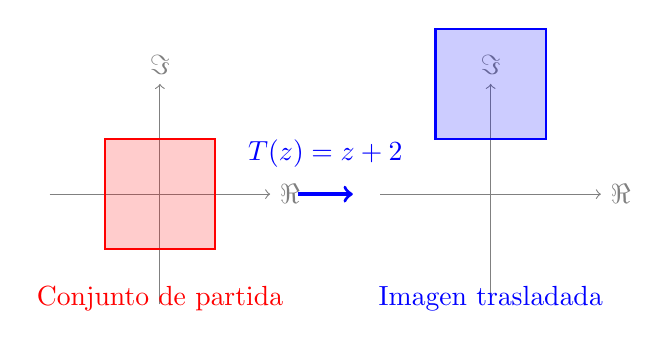
\begin{tikzpicture}[scale=0.7]
        % Conjunto de partida
        \begin{scope}[xshift=-3cm]
            \draw[->, gray] (-2,0) -- (2,0) node[right] {$\Re$};
            \draw[->, gray] (0,-2) -- (0,2) node[above] {$\Im$};
            \draw[red, thick] (-1,-1) rectangle (1,1);
            \fill[red, opacity=0.2] (-1,-1) rectangle (1,1);
            \node[red, below] at (0,-1.5) {Conjunto de partida};
        \end{scope}
        
        % Flecha de transformación
        \draw[->, blue, very thick] (-0.5,0) -- (0.5,0);
        \node[blue, above] at (0,0.3) {$T(z) = z + 2$};
        
        % Imagen
        \begin{scope}[xshift=3cm]
            \draw[->, gray] (-2,0) -- (2,0) node[right] {$\Re$};
            \draw[->, gray] (0,-2) -- (0,2) node[above] {$\Im$};
            \draw[blue, thick] (-1,1) rectangle (1,3);
            \fill[blue, opacity=0.2] (-1,1) rectangle (1,3);
            \node[blue, below] at (0,-1.5) {Imagen trasladada};
        \end{scope}
    \end{tikzpicture}
    \end{center}
    \item $T(z) = \alpha z$ con $\alpha > 0$ es una \textbf{homotecia}.
    
    \begin{center}
    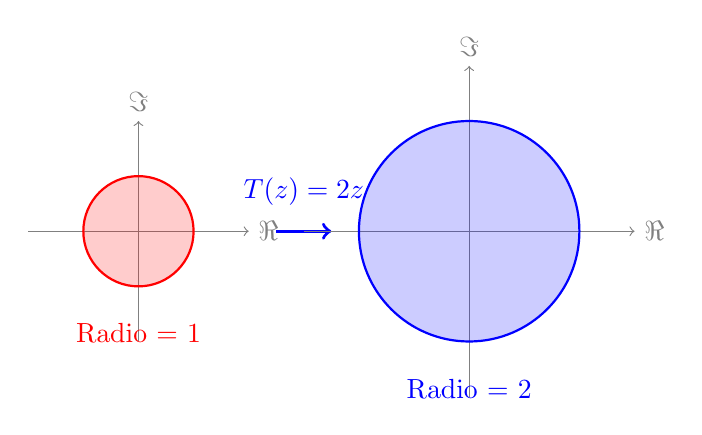
\begin{tikzpicture}[scale=0.7]
        % Conjunto de partida
        \begin{scope}[xshift=-3cm]
            \draw[->, gray] (-2,0) -- (2,0) node[right] {$\Re$};
            \draw[->, gray] (0,-2) -- (0,2) node[above] {$\Im$};
            \draw[red, thick] (0,0) circle (1);
            \fill[red, opacity=0.2] (0,0) circle (1);
            \node[red, below] at (0,-1.5) {Radio = 1};
        \end{scope}
        
        % Flecha de transformación
        \draw[->, blue, very thick] (-0.5,0) -- (0.5,0);
        \node[blue, above] at (0,0.3) {$T(z) = 2z$};
        
        % Imagen
        \begin{scope}[xshift=3cm]
            \draw[->, gray] (-3,0) -- (3,0) node[right] {$\Re$};
            \draw[->, gray] (0,-3) -- (0,3) node[above] {$\Im$};
            \draw[blue, thick] (0,0) circle (2);
            \fill[blue, opacity=0.2] (0,0) circle (2);
            \node[blue, below] at (0,-2.5) {Radio = 2};
        \end{scope}
    \end{tikzpicture}
    \end{center}
    \item $T(z) = cz$ con $|c| = 1$ es una \textbf{rotación}, pues $|c| = 1 \implies c = \cos(\theta) + i\sin(\theta) \quad \theta \in \mathbb{R}$, y por tanto:
    \[
    T(z) = cz 
    = (\cos(\theta) + i\sin(\theta))|z|(\cos(\beta) + i\sin(\beta)) =
    |z|(\cos(\theta + \beta) + i\sin(\theta + \beta)) =
    e^{i\theta}z
    \]
    
    \begin{center}
    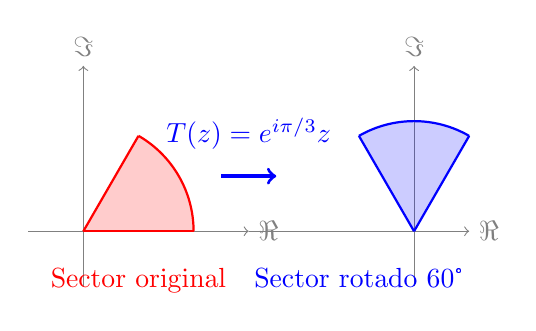
\begin{tikzpicture}[scale=0.7]
        % Conjunto de partida
        \begin{scope}[xshift=-3cm]
            \draw[->, gray] (-1,0) -- (3,0) node[right] {$\Re$};
            \draw[->, gray] (0,-1) -- (0,3) node[above] {$\Im$};
            \fill[red, opacity=0.2] (0,0) -- (2,0) arc (0:60:2) -- cycle;
            \draw[red, thick] (0,0) -- (2,0);
            \draw[red, thick] (0,0) -- (1,1.73);
            \draw[red, thick] (2,0) arc (0:60:2);
            \node[red, below] at (1,-0.5) {Sector original};
        \end{scope}
        
        % Flecha de transformación
        \draw[->, blue, very thick] (-0.5,1) -- (0.5,1);
        \node[blue, above] at (0,1.3) {$T(z) = e^{i\pi/3}z$};
        
        % Imagen
        \begin{scope}[xshift=3cm]
            \draw[->, gray] (-3,0) -- (1,0) node[right] {$\Re$};
            \draw[->, gray] (0,-1) -- (0,3) node[above] {$\Im$};
            \fill[blue, opacity=0.2] (0,0) -- (1,1.73) arc (60:120:2) -- cycle;
            \draw[blue, thick] (0,0) -- (1,1.73);
            \draw[blue, thick] (0,0) -- (-1,1.73);
            \draw[blue, thick] (1,1.73) arc (60:120:2);
            \node[blue, below] at (-1,-0.5) {Sector rotado 60°};
        \end{scope}
    \end{tikzpicture}
    \end{center}
    
    \item $T(z) = \frac{1}{z}$ es una \textbf{inversión} (respecto a la circunferencia unidad).
    
    \begin{center}
    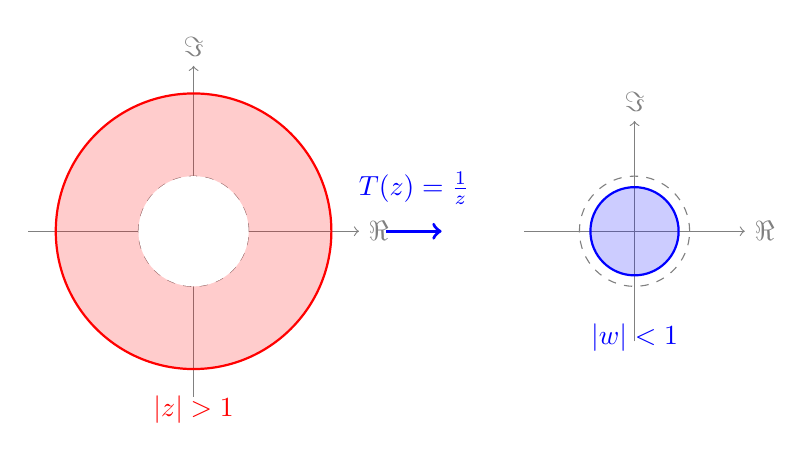
\begin{tikzpicture}[scale=0.7]
        % Conjunto de partida
        \begin{scope}[xshift=-4cm]
            \draw[->, gray] (-3,0) -- (3,0) node[right] {$\Re$};
            \draw[->, gray] (0,-3) -- (0,3) node[above] {$\Im$};
            % Circunferencia unidad de referencia
            \draw[gray, dashed] (0,0) circle (1);
            % Conjunto exterior |z| > 1
            \draw[red, thick] (0,0) circle (2.5);
            \fill[red, opacity=0.2] (0,0) circle (2.5);
            \fill[white] (0,0) circle (1);
            \node[red, below] at (0,-2.8) {$|z| > 1$};
        \end{scope}
        
        % Flecha de transformación
        \draw[->, blue, very thick] (-0.5,0) -- (0.5,0);
        \node[blue, above] at (0,0.3) {$T(z) = \frac{1}{z}$};
        
        % Imagen
        \begin{scope}[xshift=4cm]
            \draw[->, gray] (-2,0) -- (2,0) node[right] {$\Re$};
            \draw[->, gray] (0,-2) -- (0,2) node[above] {$\Im$};
            % Circunferencia unidad de referencia
            \draw[gray, dashed] (0,0) circle (1);
            % Imagen interior |w| < 1
            \draw[blue, thick] (0,0) circle (0.8);
            \fill[blue, opacity=0.2] (0,0) circle (0.8);
            \node[blue, below] at (0,-1.5) {$|w| < 1$};
        \end{scope}
    \end{tikzpicture}
    \end{center}
\end{itemize}

\begin{definición} [Homeomorfismo]
    Sea $X$ e $Y$ dos espacios topológicos. Una función $f : X \to Y$ es un \textbf{homeomorfismo} si es biyectiva, continua y su inversa $f^{-1} : Y \to X$ también es continua.
\end{definición}

\begin{observación}
    Si tenemos $a,b,c,d \in \mathbb{C}$ con $ad - bc \neq 0$, la transformación de Möbius $T(z) = \frac{az + b}{cz + d}$, podemos observar que los límites:
\[
\begin{cases}
    \lim_{z \to \infty} T(z) = 
    \lim_{z \to \infty} \frac{az + b}{cz + d} =
    \lim_{z \to \infty} \frac{a + \frac{b}{z}}{c + \frac{d}{z}} =
    \frac{a}{c}\\
    \lim_{z \to -\frac{d}{c}} T(z) = \infty
\end{cases}
\]
    Además podemos extender $T$ a todo $\overline{\mathbb{C}}$ de la siquiente forma:
\[
    T: \mathbb{C} \setminus \{-\frac{d}{c}\} \to \mathbb{C} \setminus \{\frac{a}{c}\} \longrightarrow
    T: \overline{\mathbb{C}} \to \overline{\mathbb{C}} \quad
    \begin{cases}
        -\frac{d}{c} \to \infty \\
        \infty \to \frac{a}{c} \\
        z \to T(z) \iff z \in \mathbb{C} \setminus \{-\frac{d}{c}\}
    \end{cases}
\]
Siendo así $T: \overline{\mathbb{C}} \to \overline{\mathbb{C}}$ un homeomorfismo.
\end{observación}



\begin{proposición}
    Si $T(z) = \frac{az + b}{cz + d}$ es una transformación de Möbius, entonces $T: \mathbb{C} \setminus \{-\frac{d}{c}\} \to \mathbb{C} \setminus \{\frac{a}{c}\}$ es holomorfa, biyectiva y su inversa es tambien una transformación de Möbius tal que $T^{-1}(z) = \frac{dz - b}{-cz + a}$.
\end{proposición}

\begin{proof}
    $T$ es una función racional, por tanto es un cociente de potencias, y por tanto es holomorfa en $\mathbb{C} \setminus \left\{ z : T(z) = 0 \right\} = \mathbb{C} \setminus \{-\frac{d}{c}\}$.\\
    Su derivada es:
    \[
        T'(z) = \frac{(az + b)'(cz + d) - (az + b)(cz + d)'}{(cz + d)^2} =
        \frac{acz + ad - acz + bd}{(cz + d)^2} =
        \frac{ad - bc}{(cz + d)^2} \neq 0 \quad \forall z \in \mathbb{C} \setminus \{-\frac{d}{c}\}
    \]
    Si tomamos $w = T(z)$:
    \[
    w = \frac{az + b}{cz + d} \iff
    cwz + wd = az + b \iff
    (cw - a)z = b - wd \iff
    z = \frac{-wd + b}{cw - a}
    \]
    Luego $T^{-1}(z) = \frac{-dz + b}{cz - a}$, que es una transformación de Möbius con $(-d)(-a) - b c = ad - bc \neq 0$.\\
    Además $T: \overline{\mathbb{C}} \to \overline{\mathbb{C}}$ es homeomorfismo pues lo es de $\mathbb{C} \setminus \{-\frac{d}{c}\} \to \mathbb{C} \setminus \{\frac{a}{c}\}$ y además lo hemos extendido con continuidad.
\end{proof}

\begin{proposición}
    Toda transformación de Möbius es una composición finita de traslaciones, homotecias, rotaciones e inversiones.
\end{proposición}

\begin{proof}
    Si $a \in \mathbb{C} \setminus \{0\}$, $T(z) = az$ es la composicion de una homotecia y un giro pues:
    \[
    T(z) =
    az =
    |a|(\frac{a}{|a|}z) \underbrace{=}_{\frac{a}{|a|} = e^{i\theta}}
    |a|(e^{i\theta}z) =
    (T_2 \circ T_1)(z)
    \]
    Siendo:
    \[
    \begin{cases}
        T_1(z) = e^{i\theta}z \quad \text{(rotación)} \\
        T_2(z) = |a|z \quad \text{(homotecia)}
    \end{cases} \implies
    z \xrightarrow{T_1} e^{i\theta}z \xrightarrow{T_2} |a|(e^{i\theta}z) = az
    \]
    En general, sea $T(z) = \frac{az + b}{cz + d}$ con $ad - bc \neq 0$:
    \begin{itemize}
        \item Si $c = 0$, entonces $T(z) = \frac{az + b}{d} = \frac{a}{d}z + \frac{b}{d} = (T_2 \circ T_1)(z)$ siendo $T_1(z) = \frac{a}{d}z$ (homotecia y rotación) y $T_2(z) = z + \frac{b}{d}$ (traslación).
        \item Si $c \neq 0$:
        \[
        z \xrightarrow{T_1} 
        z + \frac{d}{c} \xrightarrow{T_2} 
        \frac{1}{z + \frac{d}{c}} = \frac{c}{cz + d} \xrightarrow{T_3} 
        \frac{bc - ad}{c^2}z + \frac{c}{cz + d} \xrightarrow{T_4} 
        -\frac{bc - ad}{c^2}z + \frac{c}{cz + d} + \frac{a}{c} =
        \frac{az + b}{cz + d}
        \]
        Luego $T = T_4 \circ T_3 \circ T_2 \circ T_1$
    \end{itemize}
\end{proof}

\begin{proposición}
    Si $T$ y $S$ son transformaciones de Möbius, entonces $T^{-1}$ y $T \circ S$ son transformaciones de Möbius. Por tanto, el conjunto de todas las transformaciones de Möbius es un grupo no conmutativo respecto a la composición.
\end{proposición}

\begin{proof}
    Ya vimos en la prop 1 que $T^{-1}$ es una transformación de Möbius. Para probar que $T \circ S$ es una transformación de Möbius, tenemos que por la prop 2 basta con probarlo para $S$ siendo una traslación, homotecia, rotación o inversión. Y para cada una de estas transformaciones, es muy sencillo comprobarlo.
\end{proof}

\textbf{Nota:} La expresión de $T(z) = \frac{az + b}{cz + d}$ no es única, pues si multiplicamos numerador y denominador por una constante $\lambda \in \mathbb{C} \setminus \{0\}$, obtenemos la misma transformación:

\[
    T(z) = \frac{az + b}{cz + d} = \frac{\lambda(az + b)}{\lambda(cz + d)} = \frac{(\lambda a)z + (\lambda b)}{(\lambda c)z + (\lambda d)}
\]

\begin{proposición}
    Si $T$ es una transformación de Möbius tal que $T(z) \neq Id$, entonces $T$ tiene exactamente dos puntos fijos (aunque uno de ellos puede ser doble).
\end{proposición}

\begin{proof}
    Sea $T(z) = \frac{az + b}{cz + d}$ con $ad - bc \neq 0$. 
    \[
    T(z) = z \iff \frac{az + b}{cz + d} = z \iff az + b = z(cz + d) 
    \]
    \[
    \iff cz^2 + (d - a)z - b = 0
    \]
    \begin{itemize}
        \item Si $c \neq 0$, la ecuación 
        \[
            cz^2 + (d - a)z - b = 0
        \]
        es de segundo grado y tiene dos soluciones.
        \[
            (\alpha z^2 + \beta z + \gamma = 0) 
            \iff z^2 + \frac{\beta}{\alpha}z + \frac{\gamma}{\alpha} = 0 
            \iff z^2 + \tilde{\beta} z + \tilde{\gamma} = 0 
        \]
        \[
            \iff \left(z + \frac{\tilde{\beta}}{2}\right)^2 - \frac{\tilde{\beta}^2}{4} + \tilde{\gamma} = 0 
            \iff \left(z + \frac{\tilde{\beta}}{2}\right)^2 = \frac{\tilde{\beta}^2}{4} - \tilde{\gamma}.
        \]        
        Si $\alpha_1, \alpha_2$ son las dos raíces cuadradas de $\tfrac{\tilde{\beta}^2}{4} - \tilde{\gamma}$, entonces 
        \[
            z_1 = \alpha_1 - \frac{\tilde{\beta}}{2}, 
            \qquad 
            z_2 = \alpha_2 - \frac{\tilde{\beta}}{2}
        \]
        son las dos soluciones de la ecuación.        
        \item Si $c = 0$, entonces los puntos fijos son $\infty$ y $\frac{b}{d-a}$ (que en el caso $d=a$ este segundo punto también es $\infty$).
        \[
            T\left(\frac{b}{d-a}\right) = \frac{a\frac{b}{d-a} + b}{d} = \frac{\frac{ab}{d-a} + b}{d} = \frac{\frac{ab + bd - ab}{d-a}}{d} = \frac{\frac{bd}{d-a}}{d} = \frac{b}{d-a}
        \]
    \end{itemize}
\end{proof}

\begin{corolario}
    Si $T$ y $S$ son transformaciones de Möbius que coinciden en tres puntos distintos, entonces $T = S$.
\end{corolario}

\begin{proof}
    Basta tener en cuenta que $S^{-1} \circ T$ tiene tres puntos fijos. Por tanto por la prop 4, $S^{-1} \circ T = Id$, luego $T = S$.
\end{proof}

Si $z_1, z_2$ y $z_3$ son tres puntos distintos de $\overline{\mathbb{C}}$, entonce existe un única transformación de Möbius que lleva los puntos $z_1, z_2$ y $z_3$ en los puntos $1, 0$ y $\infty$ respectivamente. 

Podemos comprobar que esa transformación es 
\[
    S(z) = \frac{(z - z_2)/(z - z_3)}{(z_1 - z_2)/(z_1 - z_3)} \quad \text{si } z_1, z_2, z_3 \in \mathbb{C}
\]

\[
    S(z) = \frac{(z - z_2)}{(z - z_3)} \text{si } z_1 = \infty, z_2, z_3 \in \mathbb{C}
\]

\[
    S(z) = \frac{(z_1 - z_3)}{(z - z_3)} \text{si } z_2 = \infty, z_1, z_3 \in \mathbb{C}
\]

\[
    S(z) = \frac{(z - z_2)}{(z_1 - z_2)} \text{si } z_3 = \infty, z_1, z_2 \in \mathbb{C}
\]

Vamos a denotar $S_{z_1, z_2, z_3}(z)$ a la transformación anterior.



\begin{proposición}
    Dados tres puntos distintos $z_1, z_2, z_3 \in \overline{\mathbb{C}}$ y otros tres puntos distintos $w_1, w_2, w_3 \in \overline{\mathbb{C}}$, existe una única transformación de Möbius $T$ tal que $T(z_i) = w_i$ para $i = 1, 2, 3$. 
\end{proposición}

\begin{proof}
    Tenemos que 
    \[
        \begin{matrix}
            \quad & S_{z_1, z_2, z_3}(z) & \quad & S_{w_1, w_2, w_3}(z) & \quad \\
            z_1 & \longrightarrow & 1 & \longleftarrow & w_1 \\
            z_2 & \longrightarrow & 0 & \longleftarrow & w_2 \\
            z_3 & \longrightarrow & \infty & \longleftarrow & w_3
        \end{matrix}
    \]   
    Basta tomar $T = S_{w_1, w_2, w_3}^{-1} \circ S_{z_1, z_2, z_3}$.
\end{proof}


\begin{definición} [Razón doble]
    Se $z_1, z_2, z_3, z_4 \in \overline{\mathbb{C}}$ puntos distintos, se llama \textbf{razón doble} de los cuatro puntos al número complejo
    \[
        (z_1, z_2, z_3,z_4) := S_{z_2, z_3, z_4}(z_1) 
    \]
\end{definición}


\begin{teorema}
    Sean $z_2, z_3, z_4 \in \overline{\mathbb{C}}$ puntos distintos y $T$ una transformación de Möbius, entonces
    \[
        (T(z), T(z_2), T(z_3), T(z_4)) = (z, z_2, z_3, z_4) \quad \forall z \in \overline{\mathbb{C}} \setminus \{z_2, z_3, z_4\}
    \]
\end{teorema}

\begin{proof}
    Sea $z \in \overline{\mathbb{C}} \setminus \{z_2, z_3, z_4\}$,
    \[
        (T(z), T(z_2), T(z_3), T(z_4)) = S_{T(z_2), T(z_3), T(z_4)}(T(z)) = (S_{z_2, z_3, z_4} \circ T^{-1})(T(z))
    \]
    \[  
        = S_{z_2, z_3, z_4}(z) = (z, z_2, z_3, z_4)
    \]
    donde $S_{T(z_2), T(z_3), T(z_4)} = S_{z_2, z_3, z_4} \circ T^{-1}$.
\end{proof}

\begin{lema}
    Sea $T$ una transformación de Möbius, entonces $T^{-1}(\mathbb{R})$ es una circunferencia o una recta en $\mathbb{C}$ (es decir, $\{z \in \mathbb{C} : T(z) \in \mathbb{R}\}$ es una circunferencia o una recta en $\mathbb{C}$).
\end{lema}

\begin{proof}
    Sea $T(z) = \frac{az + b}{cz + d}$ con $ad - bc \neq 0$. 
    \[
        T(z) \in \mathbb{R} \iff T(z) = \overline{T(z)} \iff \frac{az + b}{cz + d} = \frac{\overline{a}\overline{z} + \overline{b}}{\overline{c}\overline{z} + \overline{d}} 
    \]
    \[
        \iff az\overline{c}\overline{z} + a\overline{d}z + b\overline{c}\overline{z} + b\overline{d} = \overline{a}\overline{z}cz + \overline{a}dz + \overline{b}cz + \overline{b}d
    \]
    \[
        \iff (a\overline{c} - \overline{a}c)z\overline{z} + (a\overline{d} - \overline{b}c)z + (b\overline{c} - \overline{a}d)\overline{z} + (b\overline{d} - \overline{b}d) = 0
    \]
    Se comprueba fácilmente que $z=-\frac{-d}{c}$ cumple la ecuación
    \begin{itemize}
        \item Si $a\overline{c} - \overline{a}c = 0$, entonces la ecuación anterior nos queda
        \[
            2 \Im(a\overline{d}z - b\overline{c}z + b\overline{d}) = 0 \iff \Im((a\overline{d} - b\overline{c})z) = \Im(b\overline{d}) = 0
        \]
        \item Suponemos que $a\overline{c} - \overline{a}c \neq 0$, entonces la ecuación anterior nos queda
        \[
            |z|^2+\frac{a\overline{d} - \overline{b}c}{a\overline{c} - \overline{a}c}z - \frac{\overline{a}d - b\overline{c}}{a\overline{c} - \overline{a}c}\overline{z} + \frac{b\overline{d} - \overline{b}d}{a\overline{c} - \overline{a}c} = 0
        \]
        Llamemos $\overline{\gamma}= \frac{a\overline{d} - \overline{b}c}{a\overline{c} - \overline{a}c}$ con lo cual $\gamma = \frac{\overline{a}d - b\overline{c}}{a\overline{c} - \overline{a}c}$
        y llamemos $\delta = \frac{b\overline{d} - \overline{b}d}{a\overline{c} - \overline{a}c} = \frac{2i \Im(b\overline{d})}{2i \Im(a\overline{c})} \in \mathbb{R}$, luego la ecuación nos queda
        \[
            |z|^2 + \gamma z - \overline{\gamma}\overline{z} + \delta = 0 \iff
            |z+\gamma|^2 - |\gamma|^2 - \delta = 0 \iff
        \]
        \[
            |z + \gamma|^2 = |\gamma|^2 - \delta \iff |z + \delta | = \sqrt{|\gamma|^2 - \delta}
        \]
        esto es la ecuación de una circunferencia de centro $-\gamma$ y radio $\sqrt{|\gamma|^2 - \delta}$.

    \end{itemize}
    
\end{proof}

\begin{proposición}
    Sean $z_1, z_2, z_3, z_4 \in \mathbb{C}$ puntos distintos, entonces son equivalentes:
    \begin{enumerate}
        \item $(z_1, z_2, z_3, z_4) \in \mathbb{R}$
        \item $z_1, z_2, z_3, z_4$ están sobre una misma circunferencia o recta.
    \end{enumerate}
\end{proposición}

\begin{proof}
    \[
        (z_1, z_2, z_3, z_4) = S_{z_2, z_3, z_4}(z_1) \in \mathbb{R} \iff z_1 \text{ está en la circunferencia o recta determinada por } z_2, z_3, z_4 \text{ ya que}
    \]
    \[
        S_{z_2, z_3, z_4}(z_2) = 0 \in \mathbb{R}, \quad S_{z_2, z_3, z_4}(z_3) = 1 \in \mathbb{R}, \quad S_{z_2, z_3, z_4}(z_4) = \infty \in \mathbb{R} 
    \]
\end{proof}

\begin{teorema}
    Sea $T$ una transformación de Möbius, entonces $T$ lleva circunferencias y rectas en circunferencias y rectas.
\end{teorema}

\begin{proof}
    Sean $z_2, z_3, z_4 \in \overline{\mathbb{C}}$ puntos distintos, entonces $z_2, z_3, z_4$ determinan una circunferencia o recta $\Gamma$.
    \[
        z \in \Gamma \iff (z, z_2, z_3, z_4) \in \mathbb{R} \iff (T(z), T(z_2), T(z_3), T(z_4)) = (z, z_2, z_3, z_4) \in \mathbb{R} 
    \]
    \[
        \iff T(z) \text{ está en la circunferencia o recta determinada por } T(z_2), T(z_3), T(z_4) \iff T(z) \in T(\Gamma)
    \]
\end{proof}

\ejemplo{
    \begin{itemize}
        \item Las rectas que pasan por la preimagen de $\infty$ se transforman en rectas.
        \[
        \begin{tikzpicture}[scale=1]
            % Dominio de partida
            \begin{scope}[xshift=-4cm]
                \draw[->] (-2,0) -- (2,0) node[right] {$x$};
                \draw[->] (0,-2) -- (0,2) node[above] {$y$};
                \draw[thick,blue] (-2,-2) -- (2,2);
                \node at (0,-2.5) {Dominio de partida};
            \end{scope}
            % Imagen
            \begin{scope}[xshift=4cm]
                \draw[->] (-2,0) -- (2,0) node[right] {$x$};
                \draw[->] (0,-2) -- (0,2) node[above] {$y$};
                \draw[thick,red] (-2,1) -- (2,-1);
                \node at (0,-2.5) {Imagen};
            \end{scope}
        \end{tikzpicture}
        \]

        \item Las rectas que no pasan por la preimagen de $\infty$ se transforman en circunferencias con centro en la imagen del simétrico (respecto de la recta) de la preimagen de $\infty$.
        \[
        \begin{tikzpicture}[scale=1]
            % Dominio de partida
            \begin{scope}[xshift=-4cm]
                \draw[->] (-2,0) -- (2,0) node[right] {$x$};
                \draw[->] (0,-2) -- (0,2) node[above] {$y$};
                \draw[thick,blue] (-2,1) -- (2,1);
                \node at (0,-2.5) {Dominio de partida};
            \end{scope}
            % Imagen
            \begin{scope}[xshift=4cm]
                \draw[->] (-2,0) -- (2,0) node[right] {$x$};
                \draw[->] (0,-2) -- (0,2) node[above] {$y$};
                \draw[thick,red] (0,0) circle(1.5);
                \node at (0,-2.5) {Imagen};
            \end{scope}
        \end{tikzpicture}
        \]

        \item Las circunferencias que pasan por la preimagen de $\infty$ se transforman en rectas.
        \[
        \begin{tikzpicture}[scale=1]
            % Dominio de partida
            \begin{scope}[xshift=-4cm]
                \draw[->] (-2,0) -- (2,0) node[right] {$x$};
                \draw[->] (0,-2) -- (0,2) node[above] {$y$};
                \draw[thick,blue] (0,0) circle(1.5);
                \node at (0,-2.5) {Dominio de partida};
            \end{scope}
            % Imagen
            \begin{scope}[xshift=4cm]
                \draw[->] (-2,0) -- (2,0) node[right] {$x$};
                \draw[->] (0,-2) -- (0,2) node[above] {$y$};
                \draw[thick,red] (-2,1) -- (2,1);
                \node at (0,-2.5) {Imagen};
            \end{scope}
        \end{tikzpicture}
        \]

        \item Las circunferencias que no pasan por la preimagen de $\infty$ se transforman en circunferencias con centro en la imagen del simétrico (respecto de la circunferencia de partida) de la preimagen de $\infty$.
        \[
        \begin{tikzpicture}[scale=1]
            % Dominio de partida
            \begin{scope}[xshift=-4cm]
                \draw[->] (-2,0) -- (2,0) node[right] {$x$};
                \draw[->] (0,-2) -- (0,2) node[above] {$y$};
                \draw[thick,blue] (0.5,0) circle(1);
                \node at (0,-2.5) {Dominio de partida};
            \end{scope}
            % Imagen
            \begin{scope}[xshift=4cm]
                \draw[->] (-2,0) -- (2,0) node[right] {$x$};
                \draw[->] (0,-2) -- (0,2) node[above] {$y$};
                \draw[thick,red] (-0.5,0) circle(1);
                \node at (0,-2.5) {Imagen};
            \end{scope}
        \end{tikzpicture}
        \]
    \end{itemize}
}

\begin{observación}
    Si $\Gamma$ y $\tilde{\Gamma}$ son dos circunferencias o rectas en $\overline{\mathbb{C}}$, existen muchas transformaciones de Möbius que llevan $\Gamma$ en $\tilde{\Gamma}$. 

    Pero si fijamos tres puntos distintos $z_1, z_2, z_3 \in \Gamma$ y tres puntos distintos $w_1, w_2, w_3 \in \tilde{\Gamma}$, entonces existe una única transformación de Möbius $T$ tal que $T(z_i) = w_i$ para $i = 1, 2, 3$.
\end{observación}

Si $\Gamma$ es una circunferencia en $\overline{\mathbb{C}}$, y tomamos tres puntos distintos $z_1, z_2, z_3 \in \Gamma$, tenemos definida una orientación en $\Gamma$, la que va de $z_1$ a $z_2$ (sin pasar por $z_3$), y de $z_2$ a $z_3$ (sin pasar por $z_1$).\\

Una orientación $z_1, z_2, z_3$ en una circunferencia $\Gamma$ de $\overline{\mathbb{C}}$ determina un lado derecho y un lado izquierdo en $\Gamma$ que definimos como:

\[
    \mathcal{D}(\Gamma, \{z_1, z_2, z_3\}) = \{ z \in \overline{\mathbb{C}} : \Im(z, z_1, z_2, z_3) > 0\}
\]
respectivamente
\[
    \mathcal{I}(\Gamma, \{z_1, z_2, z_3\}) = \{ z \in \overline{\mathbb{C}} : \Im(z, z_1, z_2, z_3) < 0\}
\]

\begin{proposición}
    Sea $\Gamma$ una circunferencia en $\overline{\mathbb{C}}$, y sea $T$ una transformación de Möbius y $z_1, z_2, z_3 \in \Gamma$ puntos distintos, entonces el lado derecho (respectivamente lado izquierdo) de $\Gamma$ respecto de $O = (z_1, z_2, z_3)$ se transforma en el lado derecho (respectivamente lado izquierdo) de $T(\Gamma)$ respecto de la orientacion $O' = (T(z_1), T(z_2), T(z_3))$.
\end{proposición}

\begin{proof}
    \[
    z \in \mathcal{D}(\Gamma, \{z_1, z_2, z_3\}) \iff
    \Im(z, z_1, z_2, z_3) > 0 
    \underbrace{\iff}_{(z, z_1, z_2, z_3) = (T(z), T(z_1), T(z_2), T(z_3))}
    \]
    \[
    \Im(T(z), T(z_1), T(z_2), T(z_3)) > 0 \iff
    T(z) \in \mathcal{D}(T(\Gamma), \{T(z_1), T(z_2), T(z_3)\})
    \]
\end{proof}

\ejemplo{
    Encuentra $T$ que lleva $\{ z : \Re (z) > 0 \}$ en $\{ z : |z| \leq 1 \}$, graficamente:
    \begin{center}
        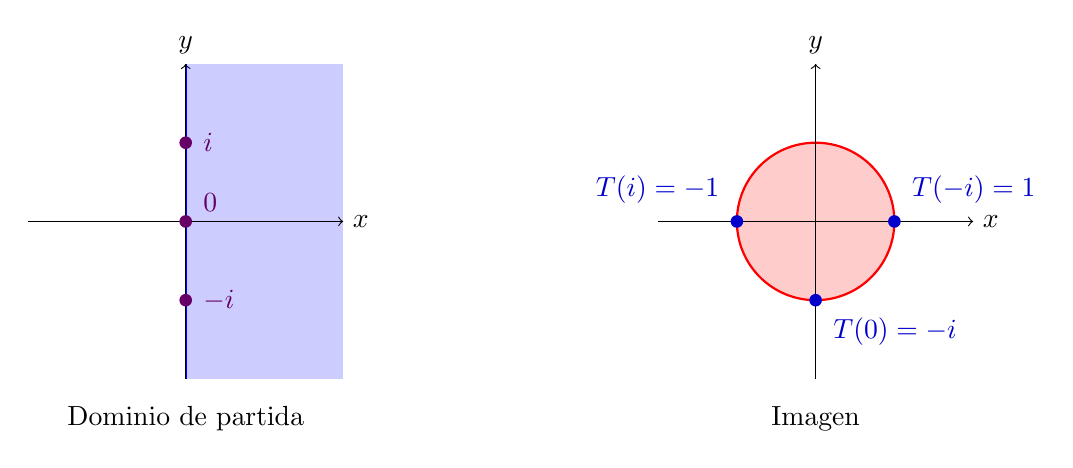
\begin{tikzpicture}[scale=1]
            % Dominio de partida
            \begin{scope}[xshift=-4cm]
                \fill[blue!20] (0,-2) -- (0,2) -- (2,2) -- (2,-2) -- cycle;
                \draw[thick,blue] (0,-2) -- (0,2);
                \node at (0,-2.5) {Dominio de partida};
                \draw[->] (-2,0) -- (2,0) node[right] {$x$};
                \draw[->] (0,-2) -- (0,2) node[above] {$y$};
                
                % Puntos específicos en violeta oscuro
                \fill[violet!80!black] (0,1) circle (0.08);
                \node[violet!80!black, right] at (0.1,1) {$i$};
                \fill[violet!80!black] (0,0) circle (0.08);
                \node[violet!80!black, above right] at (0.1,0) {$0$};
                \fill[violet!80!black] (0,-1) circle (0.08);
                \node[violet!80!black, right] at (0.1,-1) {$-i$};
            \end{scope}
            % Imagen
            \begin{scope}[xshift=4cm]
                \fill[red!20] (0,0) circle(1);
                \draw[thick,red] (0,0) circle(1);
                \node at (0,-2.5) {Imagen};
                \draw[->] (-2,0) -- (2,0) node[right] {$x$};
                \draw[->] (0,-2) -- (0,2) node[above] {$y$};
                
                % Imágenes de los puntos en azul marino
                \fill[blue!80!black] (1,0) circle (0.08);
                \node[blue!80!black, above right] at (1.1,0.1) {$T(-i) = 1$};
                \fill[blue!80!black] (0,-1) circle (0.08);
                \node[blue!80!black, below right] at (0.1,-1.1) {$T(0) = -i$};
                \fill[blue!80!black] (-1,0) circle (0.08);
                \node[blue!80!black, above left] at (-1.1,0.1) {$T(i) = -1$};
            \end{scope}
        \end{tikzpicture}\\
        Asi tenemos la transformación que lleva $-i, 0, i$ en $1, -i, -1$ respectivamente.
    \end{center}
}

\begin{definición}[Puntos simetricos]
    Si $\Gamma$ es una circunferencia en $\overline{\mathbb{C}}$, y $z_1, z_2, z_3 \in \Gamma$ puntos distintos de la misma, decimos que $z, z^* \in \overline{\mathbb{C}}$ son puntos simétricos respecto de $\Gamma$ si:
    \[
        (z, z_1, z_2, z_3) = \overline{(z^*, z_1, z_2, z_3)}
    \]
\end{definición}

\textbf{Nota:} Se puede demostrar que la definicion coincide con puntos simétricos respecto de una recta.

\subsection{Tipos de simetría}

\textbf{Simetría respecto de una recta:}
\begin{center}
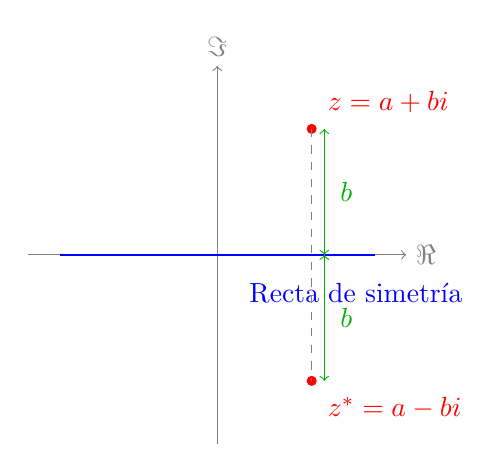
\begin{tikzpicture}[scale=0.8]
    % Ejes coordenados
    \draw[->, gray] (-3,0) -- (3,0) node[right] {$\Re$};
    \draw[->, gray] (0,-3) -- (0,3) node[above] {$\Im$};
    
    % Recta de simetría (eje real)
    \draw[thick, blue] (-2.5,0) -- (2.5,0);
    \node[blue, below] at (2.2,-0.3) {Recta de simetría};
    
    % Punto original
    \fill[red] (1.5,2) circle (0.08);
    \node[red, above right] at (1.6,2.1) {$z = a + bi$};
    
    % Punto simétrico
    \fill[red] (1.5,-2) circle (0.08);
    \node[red, below right] at (1.6,-2.1) {$z^* = a - bi$};
    
    % Línea punteada mostrando la simetría
    \draw[dashed, gray] (1.5,2) -- (1.5,-2);
    
    % Distancias iguales
    \draw[<->, green!70!black] (1.7,0) -- (1.7,2);
    \node[green!70!black, right] at (1.8,1) {$b$};
    \draw[<->, green!70!black] (1.7,-2) -- (1.7,0);
    \node[green!70!black, right] at (1.8,-1) {$b$};
\end{tikzpicture}
\end{center}

\textbf{Simetría respecto de una circunferencia:}
\begin{center}
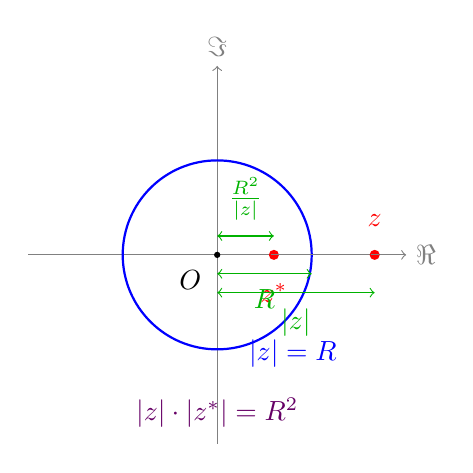
\begin{tikzpicture}[scale=0.8]
    % Ejes coordenados
    \draw[->, gray] (-3,0) -- (3,0) node[right] {$\Re$};
    \draw[->, gray] (0,-3) -- (0,3) node[above] {$\Im$};
    
    % Circunferencia de simetría (radio R)
    \draw[thick, blue] (0,0) circle (1.5);
    \node[blue, below] at (1.2,-1.2) {$|z| = R$};
    
    % Centro
    \fill[black] (0,0) circle (0.05);
    \node[black, below left] at (-0.1,-0.1) {$O$};
    
    % Punto original (exterior)
    \fill[red] (2.5,0) circle (0.08);
    \node[red, above] at (2.5,0.3) {$z$};
    
    % Punto simétrico (interior)
    \fill[red] (0.9,0) circle (0.08);
    \node[red, below] at (0.9,-0.3) {$z^*$};
    
    % Línea desde el centro
    \draw[dashed, gray] (-0.2,0) -- (2.7,0);
    
    % Radios y distancias
    \draw[<->, green!70!black] (0,-0.3) -- (1.5,-0.3);
    \node[green!70!black, below] at (0.75,-0.4) {$R$};
    \draw[<->, green!70!black] (0,0.3) -- (0.9,0.3);
    \node[green!70!black, above] at (0.45,0.4) {$\frac{R^2}{|z|}$};
    \draw[<->, green!70!black] (0,-0.6) -- (2.5,-0.6);
    \node[green!70!black, below] at (1.25,-0.7) {$|z|$};
    
    % Relación de inversión
    \node[violet!80!black] at (0,-2.5) {$|z| \cdot |z^*| = R^2$};
\end{tikzpicture}
\end{center}

\begin{teorema}[Principio de Simetría]
    Si una transformación de Möbius $T$ lleva una circunferencia $\Gamma_1$ en otra circunferencia $\Gamma_2$ de $\overline{\mathbb{C}}$, entonces $T$ lleva puntos simétricos respecto de $\Gamma_1$ en puntos simétricos respecto de $\Gamma_2$.
\end{teorema}

\begin{proof}
    Tengamos $z, z^* \in \overline{\mathbb{C}}$ puntos simétricos respecto de $\Gamma_1$, y sean $z_1, z_2, z_3 \in \Gamma_1$ puntos distintos, entonces, sabiendo que las transformaciones de Möbius preservan la razón doble:
    \[
        (z^*, z_1, z_2, z_3) = \overline{(z, z_1, z_2, z_3)} \implies
        (T(z^*), T(z_1), T(z_2), T(z_3)) =
        (z^*, z_1, z_2, z_3) = 
    \]
    \[
    = \overline{(z, z_1, z_2, z_3)} =
    \overline{(T(z), T(z_1), T(z_2), T(z_3))}
    \]
    Luego $T(z)$ y $T(z^*)$ son puntos simétricos respecto de $\Gamma_2 = T(\Gamma_1)$ que esta determinada por los puntos $T(z_1), T(z_2), T(z_3)$.
\end{proof}

Nos podemos preguntar, ¿Cúal es el simétrico del centro de una circunferencia respecto de la misma circunferencia?\\
Si la circunferencia tiene radio $r$, entonces su centro $C = 0$ está determinado por $r, ri, -r$, por lo que para que $\infty$ sea el simétrico de $C = 0$ respecto de la circunferencia, debe cumplirse que:
\[
    (\infty, r, ri, -r) = \overline{(0, r, ri, -r)}
\]
Esto se da ya que:
\[
    (0, r, ri, -r) =
    S_{r, ri, -r}(0) 
    \underbrace{=}_{
    S_{r, ri, -r}(z) = \frac{(z - ri)/(z + r)}{(r - ri)/(2r)}
    }
    =
    \frac{(2r)}{r(1-i)} \cdot \frac{-ri}{r} =
    \frac{-2i}{1-i} =
    \frac{(-2i)(1+i)}{(1-i)(1+i)} =
    1 - i =
    \overline{(0, r, ri, -r)}
\]
Por otro lado:
\[
    (\infty, r, ri, -r) =
    S_{r, ri, -r}(\infty) = 
    \frac{(2r)}{r(1-i)} = 
    \frac{2}{1-i} = 
    \frac{2(1+i)}{(1-i)(1+i)} =
    1 + i =
    \overline{(0, r, ri, -r)}
\]
Por tanto $\infty$ es el simétrico de $0$ respecto de la circunferencia $C$ de centro $0$ y radio $r$.\\
Si la circunferencia $C$ tiene centro $z_0 \neq 0$ y radio $r$, podemos tomar $S: \mathbb{C} \to \mathbb{C}$, $S(z) = z - z_0$ que lleva $C$ en la circunferencia de centro $0$ y radio $r$, luego $S(C) = \{z : |z| = r\}$, y como en $S(C)$ el simétrico de $0$ (respecto de $S(C)$) es $\infty$, entonces $S^{-1}(0)$ y $S^{-1}(\infty)$ son puntos simétricos respecto de $C$, es decir, $z_0$ y $\infty$ son puntos simétricos respecto de $C$.\\